\documentclass[a4paper]{article}
% \renewcommand{\thesection}{\Roman{section}} 

%% Language and font encodings
\usepackage[english]{babel}
\usepackage[utf8x]{inputenc}
\usepackage[T1]{fontenc}
\usepackage{float}
\usepackage{listings}
\usepackage{color}
\usepackage{subfigure}
\usepackage{graphicx}
\setlength{\parskip}{1em}


\definecolor{dkgreen}{rgb}{0,0.6,0}
\definecolor{gray}{rgb}{0.5,0.5,0.5}
\definecolor{mauve}{rgb}{0.58,0,0.82}

\lstset{frame=tb,
  language=Java,
  aboveskip=3mm,
  belowskip=3mm,
  showstringspaces=false,
  columns=flexible,
  basicstyle={\small\ttfamily},
  numbers=none,
  numberstyle=\tiny\color{gray},
  keywordstyle=\color{blue},
  commentstyle=\color{dkgreen},
  stringstyle=\color{mauve},
  breaklines=true,
  breakatwhitespace=true,
  tabsize=3
}

%% Sets page size and margins
\usepackage[a4paper,top=3cm,bottom=2cm,left=3cm,right=3cm,marginparwidth=1.75cm]{geometry}

%% Useful packages
\usepackage{amsmath}
\usepackage{graphicx}
\usepackage[colorinlistoftodos]{todonotes}
\usepackage[colorlinks=true, allcolors=blue]{hyperref}

\title{CSCE608 Project 1\\
DOTA2 STATS}
\author{Shutong Jiao 427000558}

\begin{document}
\maketitle
\section{Project Description}
The GitHub repo for this web application is https://github.com/stjiao13/Dota2Stats and the URL is https://mighty-badlands-64864.herokuapp.com/ .
\subsection{Background}
Dota 2 is a well known multiplayer online battle arena (MOBA) video game developed and published by Valve Corporation. A typical dota 2 match is played between two teams of five players, with each team occupying and defending their own separate base on the map. For each player, they control a powerful character, known as a "hero". During a match, players may collect experience points and items to increase the power of their hero and a team will win if it first destroys the opponents' base.\par
\noindent Noteworthy, a large amount of data will be generated during a dota 2 match. Therefore, data analysis for those data becomes increasingly important for players to increase their skill and also for determining if a balance update is needed. Luckily we have perfect access to these data. The detailed process of collecting data will be discussed in next section but considering this fact, it occurs to me that it would be great if we could have a website that shows recent high-level matches. 
\subsection{Functions and services of my application}

\subsubsection{Displaying all matches}
All of the matches in our web application is listed in a page. User could find many interesting statistics of a match such as duration,tower state, barrack state and match result. Besides, users could also sort matches based on all the column titles, which help user quickly find the match that they are interested in. Further, the matches table serve as an entry point as users would navigate to other tables form matches table.
\subsubsection{Displaying players profile in a match}
Like I have mentioned above, user can check players profile in a match from matches table, which is very intuitive and user-friendly. These profile includes hero name, play slot (indicate the side of a player in a match),gold, gold per minute and etc. Likewise users could also sort players based on these profile. With this information users could know more about the game and easily judge the performance of any player. Moreover, the purchase log of any player in this match is also available for user through this table.
\subsubsection{Displaying purchase log of a player in a given match}
Also, user may be curious about how a player spend his gold in a game so the purchase log is provided which consist of the name of an item and the time of purchase. This is a very useful function because this data is very important but hard to find from Dota 2 client(You need view the entire replay to find that). 
\subsubsection{Displaying teamfights in a match}
Besides, teamfights in a match is also available for user. Users could find the start and end time as well as deaths in any given teamfights. If a user wants watch the replay, he could quickly locate the period for teamfights.
\subsubsection{Leave comment for a match}
Users after viewing so many information mentioned above may want to leave a comment and luckily our website provides such application. Users could as well edit or delete a comment.

% \noindent So in my web application, users could view statistics about any match, like match duration, tower state, barrack state and result. They could also find details about players and teamfights in a given match. These statistics include hero name, gold, gold per minute, exp per minute, kills and etc. For team fights, user could see start and end time as well as number of heroes died during the team fights. Further, users may leave comment for a specific match and sort each table by columns.

\section{Data Collection}
\subsection{Data Source}
All of the data used in this project comes from Opendota, which is a volunteer-developed, open source platform providing Dota 2 data. Some of the data they provide is from the Steam WebAPI and some is from replay parsing of .dem files, which costs more time than the former.\par
\noindent Devin from Kaggle has collected a dataset containing 50000 ranked ladder matches from OpenDota. Considering the capacity of database i am using, only a small fraction of the dataset are used in my project. But it is surely effortless to import more matches into my project.\par
\subsection{Data Preprocessing}
Firstly, the initial dataset 19 different tables and not many of them are suitable for my web application. For example, 'ablility\_upgrade.csv' contains information about the ability a player choose once level up. As the maximum of level is 25 and a match has 10 players, we could expect one match have 250 corresponding entries.But usually one kind of hero has only few choices of choosing ability and thus it is meaningless to store ability upgrades with so many spaces. Another example is 'chat.csv', which is chat content per match. It does not have many unique contents (bacause chat is usually simple commands) and does not contribute much to match outcomes.\par
\noindent Then as a result, we have 6 datasets for our web application. 'matches.csv' contains top level information about each match. 'players.csv' contains totals for kills, deaths, denies, etc and player action count is also included in this dataset.'teamfights.csv' contains start and end time as well as result for every teamfights in a match. 'purchase\_log.csv' lists every item a player has purchased in a single match and this is the largest dataset in out program. 'item\_name.csv' and 'hero\_name.csv' are simply for transferring ids of item and hero to their actual name.\par
\noindent Lastly, the raw dataset contains some invalid data like duplicated ones and those are aslo excluded in the preprocessing step.
% \begin{table}
%     \centering
% \begin{tabular}{ |c|c| } 
% \hline
% filename & description \\
% \hline
% matches.csv & contains top level information about each match  \\ 
% filname2 & cell5  \\ 
% & cell8  \\ 
% \hline
% \end{tabular}
%     \caption{Caption}
%     \label{tab:my_label}
% \end{table}



% \begin{figure}[H]
% \centering
% 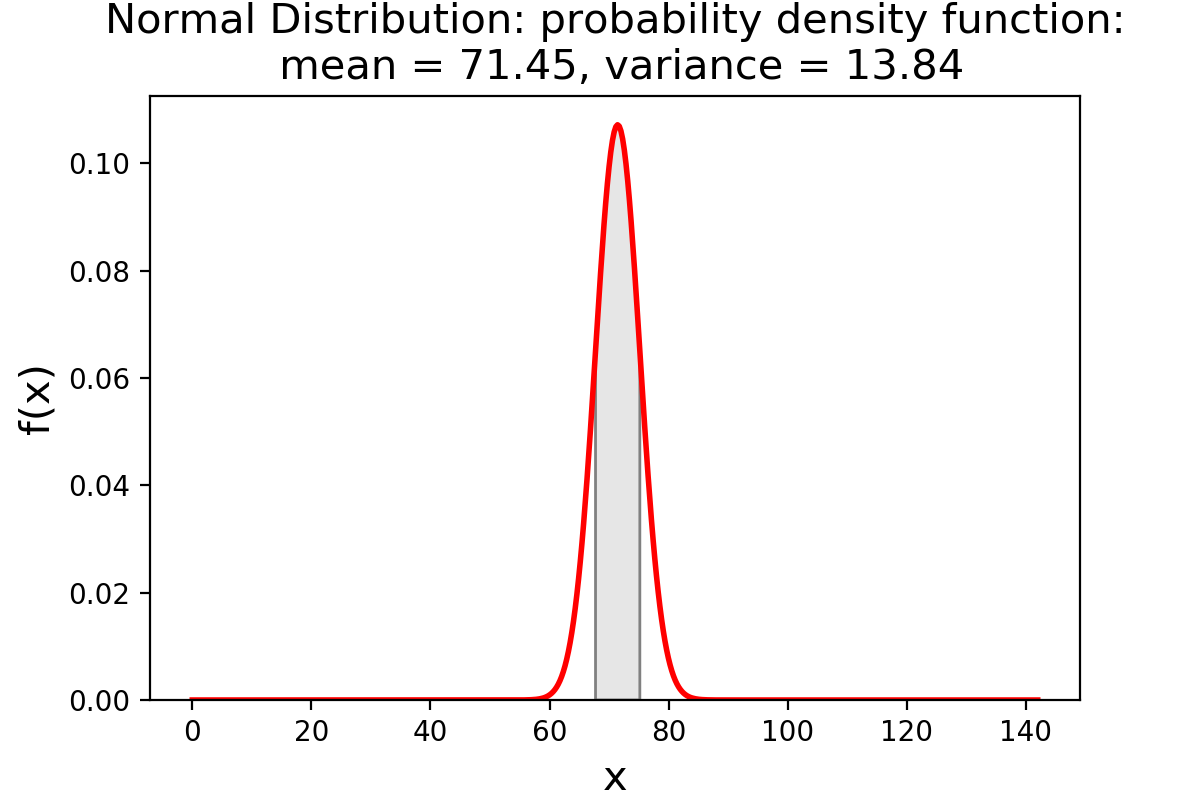
\includegraphics[width=0.8\textwidth]{1_1.png}
% % \includegraphics[width=0.8\textwidth]{1_2_50.png}
% \caption{\label{fig:fig1}probability density function of the normal distribution parameterized by the sample mean and sample variance of X}
% \end{figure}

\section{Entity Relationship Diagram}
I created the entity relationship diagram (E-R diagram) using DbSchema. The E-R diagram is shown below and I will discuss later about each table in the diagram
\begin{figure}[H]
\centering
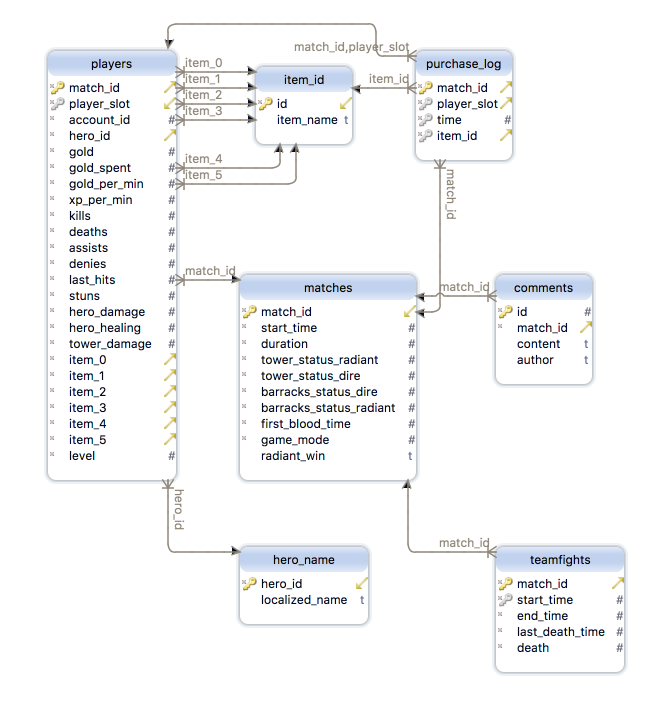
\includegraphics[width=1.0\textwidth]{erd2.png}
% \includegraphics[width=0.8\textwidth]{1_2_50.png}
\caption{Entity Relationship Diagram}
\end{figure}

\subsection{Matches}
The matches table records many key statistics of a match and it has a primary key 'match\_id', which is also foreign key in tables players, purchase\_log, comments and teamfights.
\subsection{Players}
The players table in fact set one tuple for ever player in every match. So 'account\_id' along is not a primary key. The primary key here used is ('match\_id,player\_slot'). For clarification, a dota 2 match has 10 players and 'player\_slot' indicates which slot a player is in. Another way of selecting primary key is ('match\_id,account\_id'). Theoretically, this would also work but in fact we have anonymous players in a match and the 'account\_id' is set to 0 for them. As a result, in a match there may be more than one players with 'account\_id' 0. And this is part of the reason why 'player\_slot' is very important. The 'match\_id' is also a foreign key referring to matches table.\par
\noindent Besides, item and hero name are represented as separate id in players table so that 'item\_0 - item\_5' and 'hero\_id' is also foreign key referring to item\_id and hero\_name table. We will discuss more in later corresponding part.
\subsection{Purchase\_log}
The purchase\_log table contains record for one player in a match. It stores the time and 'item\_id'. Because a player could buy multiple items at same time, the primary key here are all four attributes(match\_id, player slot, time and item\_id). Besides, match\_id and player slot is also a foreign key referring to players table.

\subsection{Teamfights}
The teamfights table contains record for every teamfight in a match. Its primary key is 'match\_id' and 'start\_time'. 'match\_id' and 'end\_time' is also a key. Even 'match\_ id' and 'last\_death\_time' could form a key. But we select the first one as primary key because it is more natural. Its foreign key is also 'match\_id' referring to matches table.
\subsection{Hero\_name}
The hero\_name table simply describes mapping between hero\_id and the localized name. Its primary is simply 'hero\_id'. And the 'hero\_id ' attribute in players table is a foreign key referring to this table.

\subsection{Item\_id}
The item\_id table , like hero\_name table, is a mapping between item\_id and item name. Its primary is simply 'id'. And any attribute from 'item\_0,...,item\_5 ' in players table is also a foreign key referring to this table.
\subsection{Comments}
The comments table stores records of every comment. The primary key is 'id' and also 'match\_id' is a foreign key referring to the matches table.

\section{Table Normalization}
The table normalization process does not change the structure of the table. Boyce-Codd normal form means that the left side of any non-trivial FD must contain a key. The reasons for why these tables are in Boyce-Codd normal form are given below:
\subsection{Matches}
We could easily observe that the left side of any FDs must contain 'match\_id'.

\subsection{Players}
Although players contains many attributes, all of the FDs have left side which is 'match\_id' and 'player\_slot'.
\subsection{Purchase\_log}
Because the primary key of purchase\_log is all four attributes, BCNF condition is automatically met.
% Clearly, we could not make FD with left side to be any combinations of 
\subsection{Teamfights}
Apparently the left side of FDs could not only contain 'death', so this is in BCNF.
\subsection{Comment}
Also it is easy to see that the FDs in comments are $id \rightarrow other\: attributes$.
\subsection{Item\_id and hero\_name}
Any two-attribute relation is in BCNF so these two tables are in BCNF.

\section{User Interface}
\subsection{Tools and Framework}
\subsubsection{Backend - Node.js}
Node.js is a widely used javascript based backend framework and it includes many helpful modules for developing. The modules I used are:
\begin{enumerate}
	\item body-parser. This module is for making the body of incoming requests possible.
	\item ejs. Known as embedded javascript templates, ejs is used as template engine for generating dynamic pages in my application.
	\item node-postgres. This is a collection of node.js modules for interfacing with PostgreSQL database.
\end{enumerate}
\subsubsection{Development Environment - Cloud 9}
I developed the web application through the IDE provided by Cloud 9, which is also a wide used cloud IDE.
\subsubsection{Frontend - Express}
Express is a minimal and flexible Node.js web application framework that provides a robust set of features for web and mobile applications.
\subsubsection{Deployment - Heroku}
Along with making development on Cloud 9, I deploy my web application on Heroku. I also used Heroku addon Heroku postgre as my PostgreSQl database.

\subsection{Interface}
\subsubsection{Landing Page}
This is the home page of my web application and users could see how many records have been stored in this website. By clicking 'Begin by browsing recent matches', user could enter the matches page.
\begin{figure}[H]
\centering
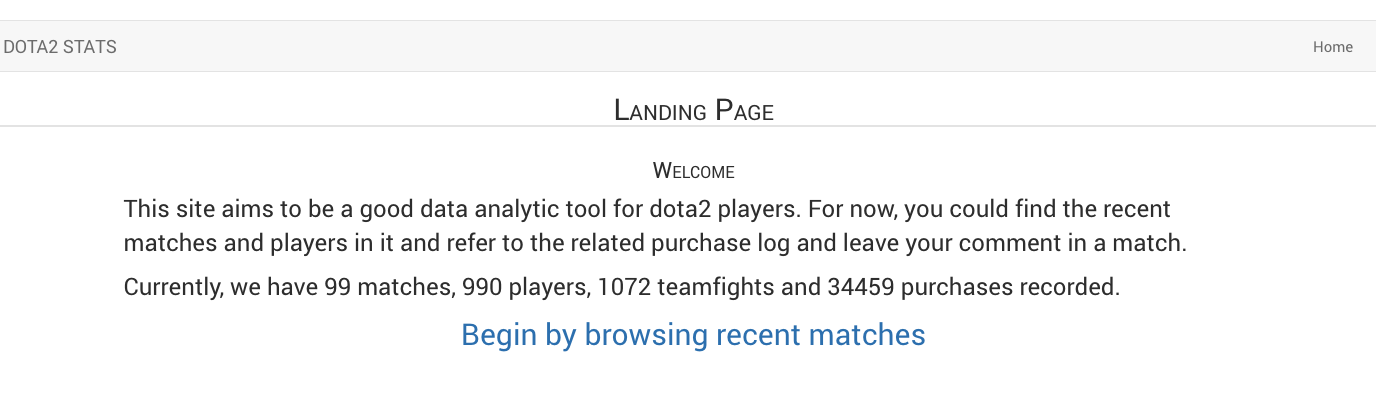
\includegraphics[width=1.0\textwidth]{landing.png}
% \includegraphics[width=0.8\textwidth]{1_2_50.png}
\caption{\label{fig:fig1}Landing page of Dota2 Stats}
\end{figure}

\subsubsection{Matches Page}
In the matches page, recent dota2 matches are shown in table as shown below:\par
\begin{figure}[H]
\centering
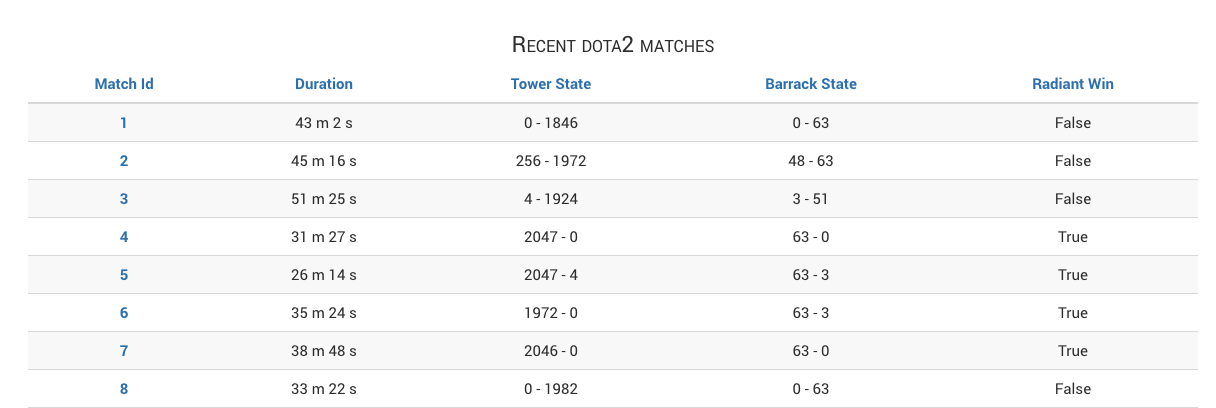
\includegraphics[width=1.0\textwidth]{matches.png}
% \includegraphics[width=0.8\textwidth]{1_2_50.png}
\caption{\label{fig:fig2}Matches page of Dota2 Stats}
\end{figure}
\noindent By clicking the title of each column title, user may see the record in ascending or descending order like shown below:

\begin{figure}[H]
\centering
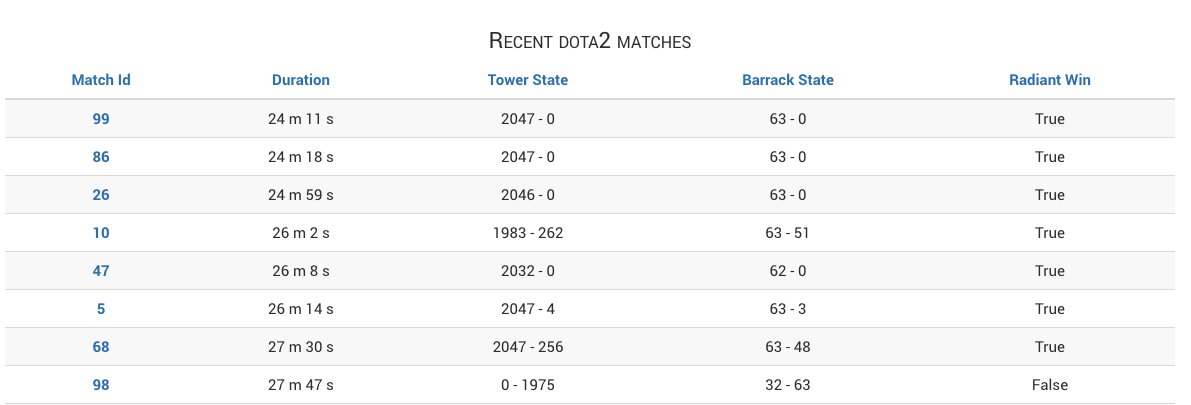
\includegraphics[width=1.0\textwidth]{matches_sort_byDuration.png}
% \includegraphics[width=0.8\textwidth]{1_2_50.png}
\caption{\label{fig:fig3}Matches page in ascending order of duration}
\end{figure}

\begin{figure}[H]
\centering
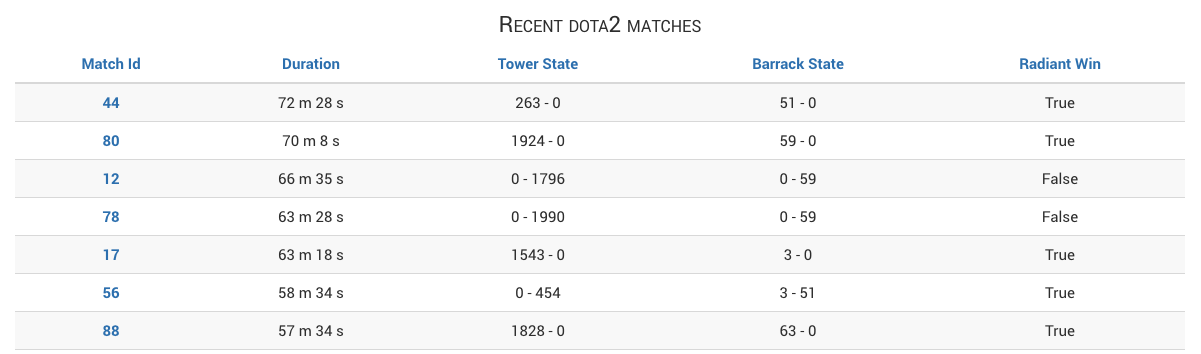
\includegraphics[width=1.0\textwidth]{matches_sort_byDuration2.png}
% \includegraphics[width=0.8\textwidth]{1_2_50.png}
\caption{\label{fig:fig4}Matches page in descending order of duration}
\end{figure}
Besides, user may see the details of a specific match in the show page by clicking the match id.

\subsubsection{Show page}
The first table in the show page lists statistics about 10 players in this game. Also users could sort the data based on column titles as shown below:\par
\begin{figure}[H]
\centering
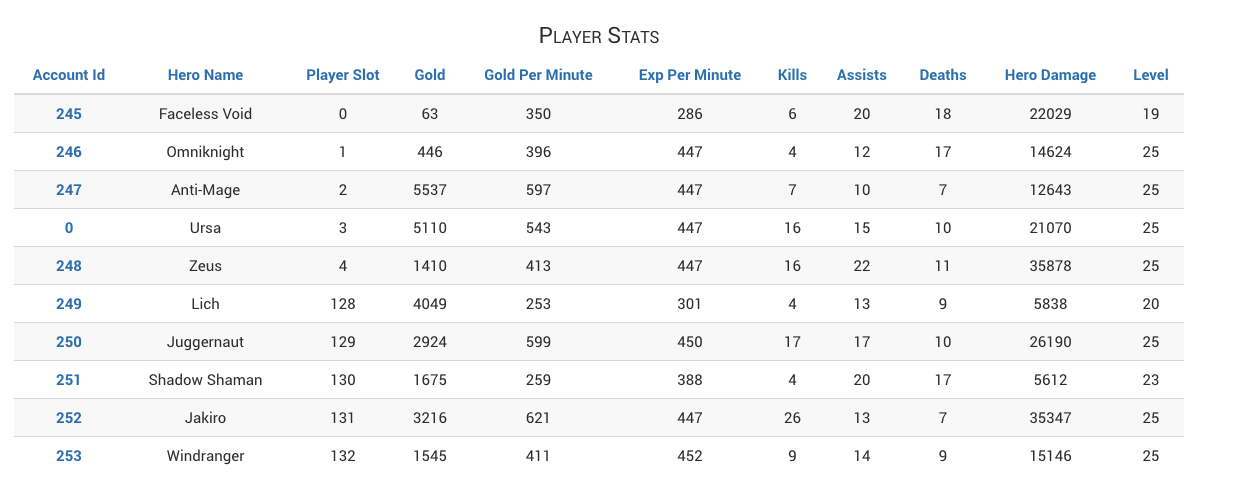
\includegraphics[width=1.0\textwidth]{show.png}
% \includegraphics[width=0.8\textwidth]{1_2_50.png}
\caption{\label{fig:fig5}Show page of player statistics}
\end{figure}

\begin{figure}[H]
\centering
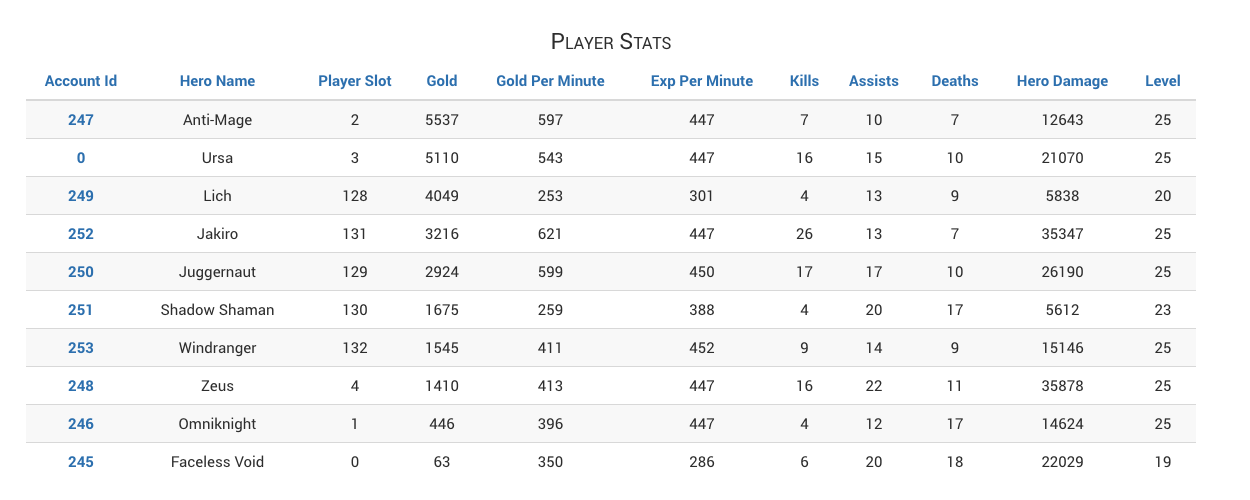
\includegraphics[width=1.0\textwidth]{show_gold_sorted.png}
% \includegraphics[width=0.8\textwidth]{1_2_50.png}
\caption{\label{fig:fig6}Show page of player statistics sorted by gold}
\end{figure}
\noindent Moreover, by clicking the account id of any player, users can view the purchase log of this player in this match as shown below:
\begin{figure}[H]
\centering
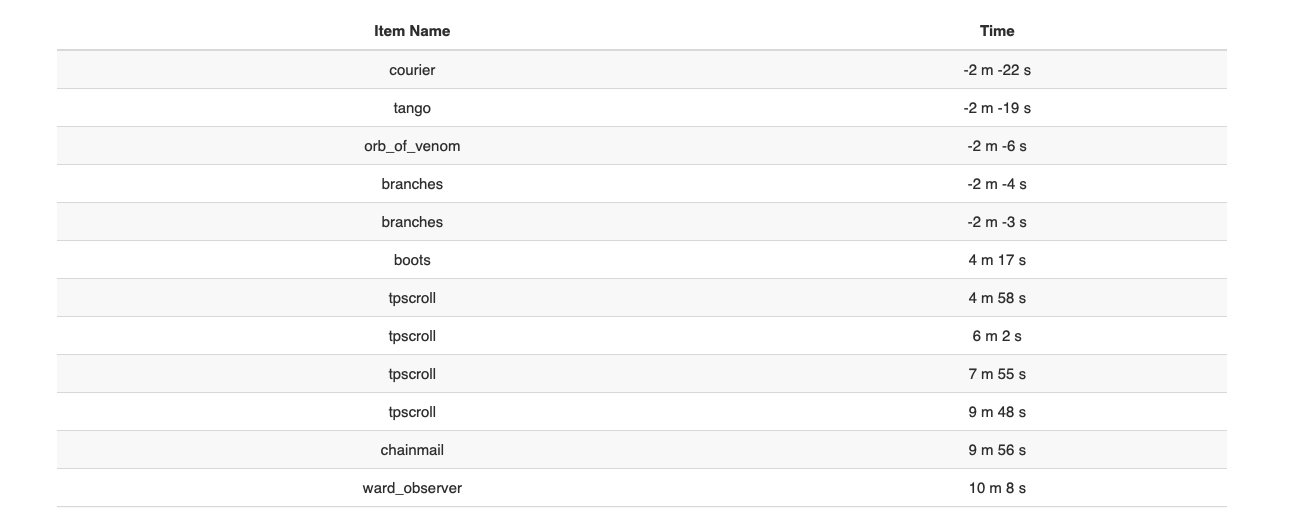
\includegraphics[width=1.0\textwidth]{purchase.png}
% \includegraphics[width=0.8\textwidth]{1_2_50.png}
\caption{\label{fig:fig7}Show page of player statistics sorted by gold}
\end{figure}

\noindent The other table that users will see in this page is the table for teamfights statistics and users will also be able to sort this table based on column title in ascending or descending order.\par
\begin{figure}[H]
\centering
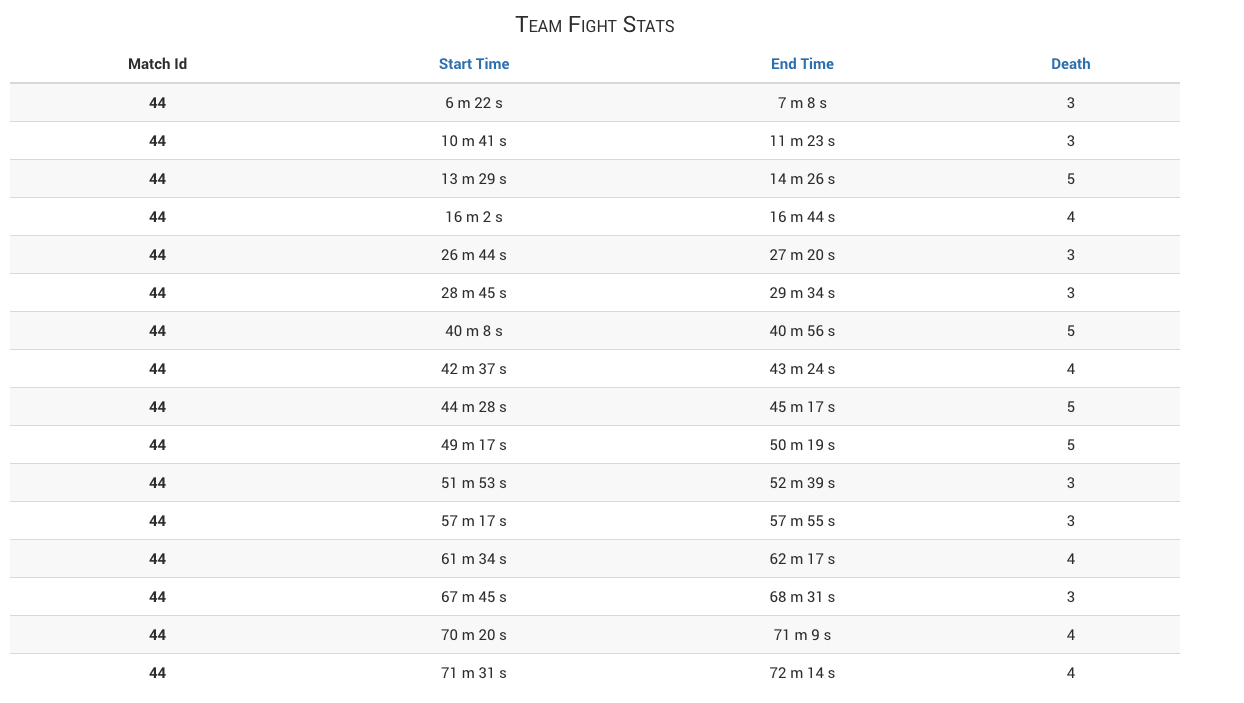
\includegraphics[width=1.0\textwidth]{teeamfight.png}
% \includegraphics[width=0.8\textwidth]{1_2_50.png}
\caption{\label{fig:fig8}Show page of player statistics}
\end{figure}
\noindent Users may leave a comment for this match at the end of page by clicking 'Add New Comment' like shown below: 
\begin{figure}[H]
\centering
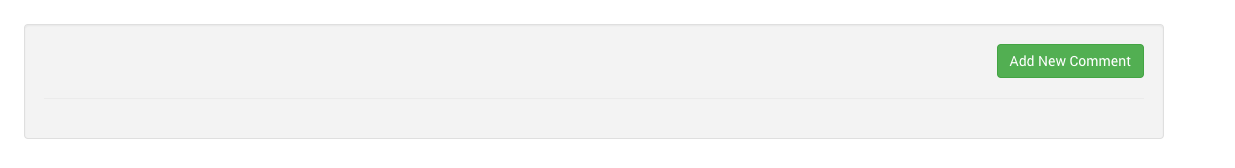
\includegraphics[width=1.0\textwidth]{add_comment2.png}
% \includegraphics[width=0.8\textwidth]{1_2_50.png}
\caption{\label{fig:fig9}Comment section in show page}
\end{figure}

\begin{figure}[H]
\centering
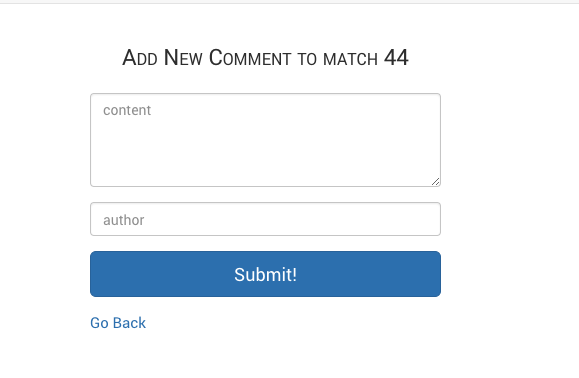
\includegraphics[width=1.0\textwidth]{comment_add.png}
% \includegraphics[width=0.8\textwidth]{1_2_50.png}
\caption{\label{fig:fig10}Add new comment page}
\end{figure}

\noindent After leaving a comment, users will be automatically directed to the original show page and see the comment he just submitted.

\begin{figure}[H]
\centering
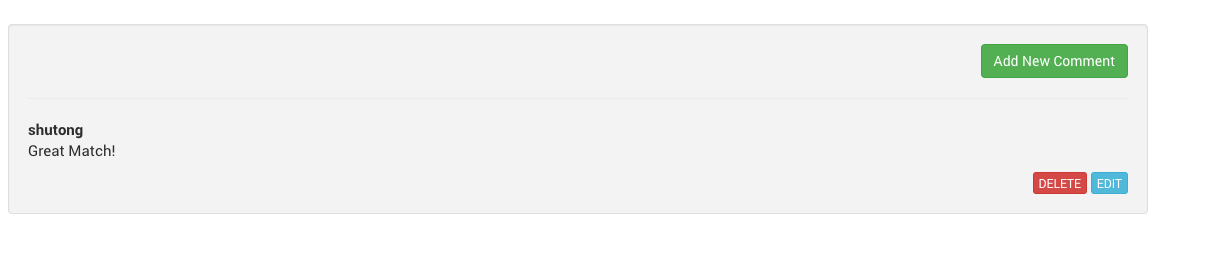
\includegraphics[width=1.0\textwidth]{comment1.png}
% \includegraphics[width=0.8\textwidth]{1_2_50.png}
\caption{\label{fig:fig11}Add new comment page}
\end{figure}

\noindent Users may also delete or edit a comment by clicking the corresponding button. Users will be directed to an edit page if edit button is clicked as shown below:

\begin{figure}[H]
\centering
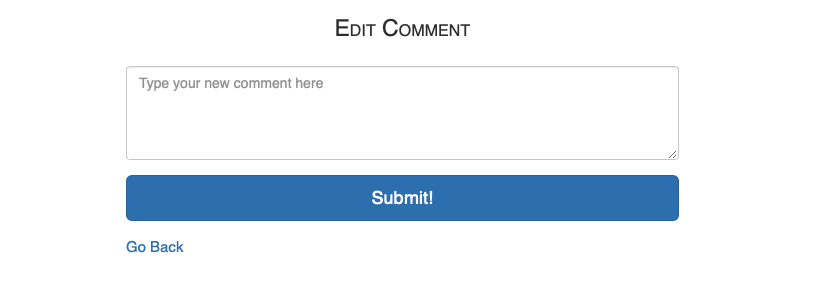
\includegraphics[width=1.0\textwidth]{edit.png}
% \includegraphics[width=0.8\textwidth]{1_2_50.png}
\caption{\label{fig:fig12}Edit page for an existing comment}
\end{figure}

\noindent Once the edit is completed, users will also be redirected to the previous show page.
\section{Project Source Code}
\subsection{SQL script as DDL}
The way I use SQL script as DDL is as following: \par
\noindent First, create related tables. The CLI command is
\begin{lstlisting}
$ psql -h MYHOST  -p MYPORT -d MYDATABASE -U MYUSERNAME -f SQLSCRIPT
\end{lstlisting}
Then,import data from csv file use 'copy' command. The CLI command for this step is 
\begin{lstlisting}
$ PGPASSWORD=PWHERE psql -h HOSTHERE -U USERHERE DBNAMEHERE -c "\copy my_things FROM 'my_data.csv' WITH CSV;"
\end{lstlisting}
And a sample of such SQL script is like : 
\begin{lstlisting}
DROP TABLE IF EXISTS comments
CREATE TABLE comments
(
  id serial NOT NULL,
  match_id serial NOT NULL,
  content text,
  author character varying(50),
  PRIMARY KEY (id),
  CONSTRAINT constraint_fk1 FOREIGN KEY (match_id) REFERENCES matches(match_id)
)
\end{lstlisting}
You could also refer to
\begin{lstlisting}
 /dota2stat/model/seed_step.txt
\end{lstlisting}
for more details.

\subsection{SQL script as DML}
All the SQL query executed in my application is defined in app.js and its code will be pasted below. You could see that most of them are INSERT, UPDATE, DELETE,COUNT and WHERE clause.
\begin{lstlisting}
var express = require("express");
var app = express();
var bodyParser  = require("body-parser");
// module for database info like password and will be ignored for public github account
var connection = require("./connection");

app.use(bodyParser.urlencoded({extended: true}));
app.use(express.static(__dirname + "/public"));

app.set("view engine","ejs");


const { Pool, Client } = require('pg')
const connectionString = connection.uri;
const router = express.Router();
const matches = [];
var sort_status = [];

// const client = new Client({
//   connectionString: connectionString,
//   ssl: true,
// });
const pool = new Pool({
  connectionString: connectionString,
  ssl: true,
});
// client.connect();


// get route for landing page
app.get("/",function(req,res) {
    var prefix = 'SELECT COUNT(*) FROM ';
    pool.query(prefix + 'matches;').then(matchesCount => {
        pool.query(prefix + 'players;').then(playersCount => {
            pool.query(prefix + 'teamfights;').then(teamfightsCount => {
                pool.query(prefix + 'purchase_log;').then(purchasesCount => {
                    
                    res.render("landing",{
                        matchesCount : matchesCount.rows[0].count,
                        playersCount : playersCount.rows[0].count,
                        teamfightsCount : teamfightsCount.rows[0].count,
                        purchasesCount : purchasesCount.rows[0].count
                    });

                })
            })
        })
    }).catch(e => console.error(e.stack));
});

// get route for matches page
app.get("/matches",function(req,res) {

    pool.query('SELECT * FROM matches;').then(matches => {
                    res.render("matches",{matches:matches.rows})
    }).catch(e => console.error(e.stack));
});

app.get("/matches/sort/:cond",function(req, res) {
    const cond = req.params.cond;
    if(sort_status[cond] === undefined) {
        sort_status[cond] = true;
    }
    else {
        sort_status[cond] = !sort_status[cond];
    }
    var text = 'SELECT * FROM matches'
    if (cond === 'byId') {
        text = 'SELECT * FROM matches ORDER BY match_id ' + (sort_status[cond] ? ' ASC ;' : ' DESC ;');
    } 
    else if (cond === 'byDuration' )  {
        text = 'SELECT * FROM matches ORDER BY duration ' + (sort_status[cond] ? ' ASC ;' : ' DESC ;');
    }
    else if (cond === 'byTower') {
        text = 'SELECT * FROM matches ORDER BY (tower_status_radiant - tower_status_dire) ' + (sort_status[cond] ? ' ASC ;' : ' DESC ;');
    }
    else if (cond === 'byBarrack') {
        text = 'SELECT * FROM matches ORDER BY (barracks_status_radiant - barracks_status_dire) ' + (sort_status[cond] ? ' ASC ;' : ' DESC ;');
    }
    else if (cond === 'byWin') {
        text = 'SELECT * FROM matches ORDER BY radiant_win ' + (sort_status[cond] ? ' ASC ;' : ' DESC ;');
    }

    pool.query(text).then(matches => {
                    res.render("matches",{matches:matches.rows})
    }).catch(e => console.error(e.stack));
}) 

// get route for show page after sorting
app.get("/matches_sorted/:id/:table/:cond",function(req, res) {
    const cond = req.params.cond;

    if(sort_status[cond] === undefined) {
        sort_status[cond] = true;
    }
    else {
        sort_status[cond] = !sort_status[cond];
    }
    if (req.params.table == 'sortByTeamfights') {
        var text1 = 'SELECT * FROM teamfights WHERE match_id = ' + req.params.id + ' ORDER BY ' + cond + (sort_status[cond] ? ' ASC ;' : ' DESC ;');
    }
    else {
        var text1 = 'SELECT * FROM teamfights WHERE match_id = ' + req.params.id +';';
    }
    if (req.params.table == 'sortByPlayers') {
        var text2 = 'SELECT * FROM players WHERE match_id = ' + req.params.id + ' ORDER BY ' + cond + (sort_status[cond] ? ' ASC ;' : ' DESC ;');
    }
    else {
        var text2 = 'SELECT * FROM players WHERE match_id = ' + req.params.id +';';
    }

    const text3 = 'SELECT * FROM comments WHERE match_id = '+ req.params.id +';';
    const text4 = 'SELECT * FROM hero_name'

    pool.query(text1).then(teamfights => {
        pool.query(text2).then(players => {
            pool.query(text3).then(comments => {
                pool.query(text4).then(hero_name => {
                    res.render("show",{
                        teamfights:teamfights.rows,
                        players:players.rows,
                        comments:comments.rows,
                        hero_name:hero_name.rows
                    })                    
                })

            })
        })
    }).catch(e => console.error(e.stack))
})

// get route for show page
app.get("/matches/:id",function(req, res) {
    const text1 = 'SELECT * FROM teamfights WHERE match_id = ' + req.params.id +';';
    pool.query(text1).then(teamfights => {
        const text2 = 'SELECT * FROM players WHERE match_id = ' + req.params.id +';';
        pool.query(text2).then(players => {
            const text3 = 'SELECT * FROM comments WHERE match_id = '+ req.params.id +';';
            pool.query(text3).then(comments => {
                const text4 = 'SELECT * FROM hero_name'
                pool.query(text4).then(hero_name => {
                    res.render("show",{
                        teamfights:teamfights.rows,
                        players:players.rows,
                        comments:comments.rows,
                        hero_name:hero_name.rows
                    })                    
                })

            })
        })
    }).catch(e => console.error(e.stack))
})

// get route for purchase page
app.get("/purchases/:id",function(req, res) {
    const id = req.params.id;
    const arr = id.split('_');
    const text1 = 'SELECT * FROM purchase_log WHERE match_id = ' + arr[0]+' AND player_slot = ' + arr[1];
    
    pool.query(text1).then(purchase_log => {
        const text2 = 'SELECT * FROM item_id;'
        pool.query(text2).then(item_id => {

            const dict = [];
            item_id.rows.forEach((value) =>{
                dict[value['id']] = value['item_name'];
            })
            res.render("purchases",{purchase_log : purchase_log.rows,
                item_id : dict
            });
        })
    }).catch(e => console.error(e.stack))
})

// get route for purchase page
app.get("/matches/:id/comments/new",function(req, res) {
   res.render("newcomment",{id:req.params.id});
})

// post route for creating new comments
app.post("/matches/:id",function(req,res) {

    
    const id = req.params.id;
    const content = req.body.comment.content;
    const author = req.body.comment.author;
    const text = 'INSERT INTO comments (match_id, content, author) VALUES ($1,$2,$3)'
    const values = [id,content,author];
    
    
    pool.query(text,values).then(created => {
        res.redirect("/matches/"+id);
    }).catch(e => console.error(e.stack))

    
})

//get route for deleting comments
app.get("/matches/:id/comments/delete/:commentId",function(req,res) {
    const text = 'delete FROM comments WHERE id = ' + req.params.commentId;
    pool.query(text).then(success => {
        res.redirect("/matches/" + req.params.id)
    }).catch(e => console.error(e.stack))
}) 

// get route for comment edit page
app.get("/matches/:id/comments/:commentId/edit",function(req,res) {
    const text = 'SELECT * FROM comments WHERE id = '+ req.params.commentId +';';
    pool.query(text).then(comment => {
        res.render("edit",{comment : comment.rows[0]});
    }).catch(e => console.error(e.stack))

})
// post route for updating existing comments
app.post("/matches/:id/comments/:commentId",function(req, res) {
    const commentId = req.params.commentId;
    const matchId = req.params.id;
    const updatedContent = req.body.comment.content;

    const text = 'UPDATE comments SET content = \'' + updatedContent +'\' WHERE id = ' + commentId +';';
    console.log(text);
    pool.query(text).then(success => {
        res.redirect("/matches/" + matchId);
    }).catch(e => console.error(e.stack))
})


app.listen(process.env.PORT,process.env.IP,() =>{
    console.log("started");
});


\end{lstlisting}
\section{Discussion}
\subsection{Data collection}
The data collection step is rather easy and the only challenge is to read though the document figuring the meaning of each attributes and deciding which to include;
\subsection{Database Design}
The original dataset are already in BCNF so I do not need to do table normalization. At first I was not very familiar with definition of primary key and foreign key and I made some mistakes. For example, I did not realize that 'match\_id' and 'player\_slot' is also a foreign key referring to players table. And i am pretty sure the current table structure is far from perfect. As I have more experience and dive deeper in database design I am sure that I am able to design a much better structure.
\subsection{Seeding the database}
This should be a rather easy step as PostgreSQL has a very good support for importing csv file using copy command. But I actually I have met much challenges and the main reason for that is heroku postgre does not give me permission for using copy command. I have also found that many users met the same problem and the only solution I have found is using direct psql command rather than an script in command line.
\subsection{Connecting to database}
I connect my web application to heroku postgre database using node-postgre. At first, the connection is done in a callback way and in the case of multiples queries the nested callback function is hard to read and maintain. This problem is also known as 'callback hell'. Node-postgre offers two other ways instead of callback function, the first is promise and the other is async/await. I choose promise because promise is easier and maintain. \par
\noindent Another issue I face is connection pooling. This is strongly recommended for web applications that make frequent queries, like ours. The reason for connection pooling is such:
\begin{enumerate}
	\item Greatly reducing the time cost by frequent queries.
	\item PostgreSQL server may crash if there are an unbounded number of connections
	\item PostgreSQL can only process one query at a time on a single connected client in a first-in first-out manner.
\end{enumerate}
And luckily node-postgres has built-in connection pooling via the pg-pool module.
\section{References}
\begin{enumerate}

	\item Dota 2. (2018, October 07). Retrieved from https://en.wikipedia.org/wiki/Dota\_2
	\item Dota 2 Matches. (n.d.). Retrieved from https://www.kaggle.com/devinanzelmo/dota-2-matches/home
	\item B. (2018, October 03). Brianc/node-postgres. Retrieved from https://github.com/brianc/node-postgres
	
\end{enumerate}







\end{document}